\chapter{Solvers and models}\label{ch:solvers}

This chapter gives the principle behind each choice of the templates and the file
where each value is. Read the values in the files.

\section{Two solvers}\label{sec:two-solvers}

\begin{tabularx}{\linewidth}{@{}P{0.20\linewidth} L L@{}}
\toprule
 & \file{case-pimple/}: \cmd{rhoPimpleFoam} & \file{case-central/}: \cmd{rhoCentralFoam} \\
\midrule
Formulation & Pressure-based, \ent{transonic} pressure equation & Density-based, explicit, central-upwind flux \\
Use & $M < 1$; start of each $M > 1$ chain & $M > 1$ \\
\bottomrule
\end{tabularx}

\medskip
The numerical dissipation of a central-upwind flux scales with the speed of sound, not
with the flow speed. At low Mach numbers it is thus large compared with the convective
flux, and the drag error grows. A pressure-based solver does not have this problem, but
it loses accuracy where strong shocks occur. The OpenFOAM ToolChain report
\citep[§6]{toolchain2026} measured both effects on rockets. The workflow therefore
changes solver at $M = 1$.

\begin{caution}
The change of discretization at $M = 1$ can cause a step in $C_D(M)$ that is not
physical. To measure it, run one Mach number with both solvers on the same mesh.
\end{caution}

The models, the gas, the boundary conditions, the function objects and the flight
condition are the same files in the two templates: \file{case-pimple/} holds only the
files that differ (\cref{sec:pimple}).

\section{Files of the templates}

\begin{longtable}{@{}P{0.40\linewidth} P{0.52\linewidth}@{}}
\caption{Files of the templates and their function.}\label{tab:template-files}\\
\toprule
File & Function \\
\midrule
\endfirsthead
\toprule
File & Function \\
\midrule
\endhead
\file{system/flowConditions} & The flight condition: the only input of a case (\cref{sec:flow-conditions}). \\
\file{system/flowDerived} & Values derived from \file{flowConditions} with \texttt{\#eval}. \\
\file{config.json} & Courant ramp and stop criterion; \file{newCase.sh} renders the \file{*.j2} files with it. \\
\file{0.orig/} & Boundary and initial conditions (\cref{sec:bc}). \\
\file{constant/thermophysicalProperties} & Gas model (\cref{sec:thermo}). \\
\file{constant/turbulenceProperties} & Turbulence model (\cref{sec:turbulence}). \\
\file{system/controlDictBase.j2}, \file{FOs/FOcommon} & Time control and function objects (\cref{sec:function-objects}). \\
\file{system/fileUpdater.j2}, \file{fileUpdaterControlDict/} & The Courant ramp of the central template (\cref{sec:ramp}). \\
\file{system/FOs/FOrunTimeControl.j2} & Stop criterion (\cref{sec:stop-criterion}). \\
\file{system/fvSchemes*}, \file{system/fvSolution} & Schemes and linear solvers (\cref{sec:schemes}). \\
\bottomrule
\end{longtable}

\begin{caution}
Use \cmd{foamDictionary -set} only on \file{flowConditions}. On a file with
\texttt{\#include} or \texttt{\#eval}, it writes the expanded values, and the file stops
following \file{flowConditions}.
\end{caution}

\section{Flight condition}\label{sec:flow-conditions}

\file{flowConditions} holds $M_\infty$, $p_\infty$, $T_\infty$, $\alpha$, $\beta$, the
turbulence intensity $T_i$ and the ratio $\nu_t/\nu$ of the free stream.
\file{flowDerived} calculates from them:
\[
  a_\infty = \sqrt{\gamma R T_\infty},\quad
  U_\infty = M_\infty a_\infty,\quad
  \rho_\infty = \frac{p_\infty}{R T_\infty},\quad
  \mu_\infty = \frac{A_s\sqrt{T_\infty}}{1 + T_s/T_\infty},
\]
\[
  k_\infty = \tfrac32 (U_\infty T_i)^2,\quad
  \nu_{t\infty} = \frac{\nu_t}{\nu}\,\nu_\infty,\quad
  \omega_\infty = \frac{k_\infty}{\nu_{t\infty}},
\]
and the velocity, drag and lift directions from $\alpha$ and $\beta$ (wind axes). The
free-stream turbulence is small and the eddy-viscosity ratio of order one, so that the
free stream does not change the boundary layer.

\section{Numerical method of rhoCentralFoam}

\cmd{rhoCentralFoam} advances the conserved variables $\rho$, $\rho\mathbf{U}$ and
$\rho E$ explicitly, then corrects the diffusive terms implicitly. It solves no
pressure equation.

\paragraph{Flux.} The central-upwind scheme of Kurganov
\citep{kurganov2000,kurganov2001} weights the face flux with the local one-sided wave
speeds. It captures shocks without a Riemann solver and without artificial viscosity.
\citet{greenshields2010} give its implementation in OpenFOAM.

\paragraph{Reconstruction.} The primitive variables go to the faces with the van Leer
TVD limiter \citep{vanleer1979}: second order in smooth regions, first order at a
discontinuity, so no new extrema occur at shocks.

\section{Local time step, Courant ramp and stop criterion}

\subsection{Local time step}\label{sec:lts}

The templates solve a steady problem with a pseudo-transient march (\ent{ddt
localEuler}). Each cell advances with the largest time step that its own Courant number
permits. The intermediate states are not physical; the converged state is. The cost
then depends on the number of iterations, not on the smallest cell of the mesh, which
with a global step sets the step of the whole domain.

\ent{deltaT} is 1, so the time counts iterations: \ent{endTime}, the write interval,
the ramp and the stop criterion are in iterations. The central template reads the
local-step controls in \file{controlDict}, the pimple template in the \ent{PIMPLE}
dictionary of \file{fvSolution}.

\begin{caution}
With \ent{localEuler}, the Courant number that \cmd{rhoCentralFoam} writes uses the
global \ent{deltaT}, not the local step: it is meaningless. Read the line
\val{Flow time scale min/max}: its minimum is the step of the most restrictive cell, and
a sudden decrease shows a cell that diverges.
\end{caution}

\subsection{Courant ramp (central template)}\label{sec:ramp}

A uniform free stream on a no-slip wall is a strong impulsive start. The explicit
central solver has no damping of the local step, so a large Courant number at the
start makes the solution leave the physical range. The ramp \citep[§5.4.1]{toolchain2026}
starts with a small Courant number and first-order reconstruction, increases the
Courant number step by step, then changes to second order and ramps again
(\cref{fig:ramp}). The function objects \ent{timeActivatedFileUpdate} copy a new
\file{controlDict} or \file{fvSchemes} at each switch; \ent{runTimeModifiable} makes the
solver read it.

\begin{figure}[htbp]
  \centering
  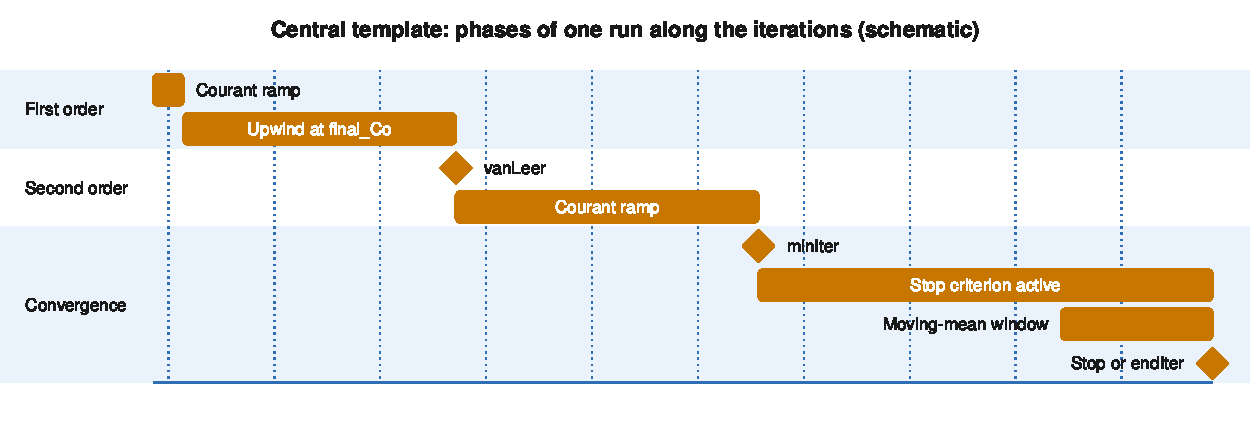
\includegraphics[width=\linewidth]{figures/pdf/ramp.pdf}
  \caption{Phases of a run of the central template along the iterations. The diamonds are the keys of \texttt{config.json} that place each switch.}
  \label{fig:ramp}
\end{figure}

The final Courant number never comes before the end of the ramp: a jump of the Courant
number makes the explicit solver fail some iterations later. The pimple template has
no ramp: its implicit pressure-velocity coupling damps the start.

\subsection{config.json}\label{sec:config-json}

\begin{tabularx}{\linewidth}{@{}P{0.26\linewidth} L@{}}
\toprule
Key & Function \\
\midrule
\ent{maxCo} (pimple), \ent{final_Co} (central) & Courant number of the converged phase. \\
\ent{vanLeer} (central) & Iteration of the change from first to second order. \\
\ent{minIter} & First iteration of the stop criterion. In the central template, also the change to the final Courant number. \\
\ent{endIter} & Last iteration if the criterion does not stop the run. \\
\ent{coeffs_fields}, \ent{coeffs_variation}, \ent{coeffs_window} & Coefficients, absolute tolerances and window of the stop criterion. \\
\bottomrule
\end{tabularx}

\medskip
The schedule comes from the ToolChain, which used another rocket. Adjust it from the
first runs: the iteration at which $C_D$ becomes flat in first order, and the
iterations that the second order needs.

\subsection{Stop criterion}\label{sec:stop-criterion}

For each coefficient $C$ in \ent{coeffs_fields}, \ent{runTimeControl} calculates the
moving mean $\overline{C}$ over \ent{coeffs_window} iterations, from \ent{minIter}. The
run stops when the window is complete and
\[
  |\overline{C} - C| < \texttt{coeffs\_variation}
\]
for all coefficients. Set the tolerance as a fraction of the expected coefficient: an
absolute tolerance is a smaller fraction of a large coefficient. The tolerance is
absolute, so it also works for a coefficient near zero, such as $C_L$ at $\alpha = 0$.
At $\alpha \neq 0$, add $C_L$ and $C_m$ to the criterion, or examine that they are flat.

To change the tolerance of a running case, edit \ent{tolerance} in its
\file{system/FOs/FOrunTimeControl} and \cmd{touch system/controlDict}. The mean then
starts again from zero.

\section{Turbulence}\label{sec:turbulence}

RANS with the $k$--$\omega$ SST model \citep{menter1994}, in the version of
\citet{menter2003} that OpenFOAM uses. The Boussinesq hypothesis gives the Reynolds
stress from an eddy viscosity,
\[
  -\overline{u_i'u_j'} = \nu_t\left(\frac{\partial U_i}{\partial x_j} + \frac{\partial U_j}{\partial x_i}\right) - \tfrac23 k\,\delta_{ij},
  \qquad
  \nu_t = \frac{a_1 k}{\max(a_1\omega,\ S F_2)}.
\]
The shear-stress limiter in the denominator limits $\nu_t$ in adverse pressure
gradients, which occur on the boattail and at the fin-body junction and set the base
flow. When you compare with the literature, find which SST version the source uses.

\subsection{Wall treatment}\label{sec:wall-treatment}

\begin{tabularx}{\linewidth}{@{}l P{0.34\linewidth} L@{}}
\toprule
Field & Condition & Principle \\
\midrule
\ent{nut} & \ent{nutUSpaldingWallFunction} & Spalding's law \citep{spalding1961} is one formula from the viscous sublayer through the buffer layer to the log layer, so it is valid for any \yplus{} of the first cell. \\
\ent{k} & \ent{kLowReWallFunction} & Also continuous in \yplus. \\
\ent{omega} & \ent{omegaWallFunction} & Blends the sublayer and log-layer values. \\
\ent{alphat} & \ent{compressible::alphatWallFunction} & Turbulent heat diffusivity from $\nu_t$ and $Pr_t$. \\
\bottomrule
\end{tabularx}

\medskip
A \yplus-insensitive wall treatment is necessary, because one mesh gives different
\yplus{} at different Mach numbers (\cref{sec:layers}). The conditions need wall
patches of type \val{wall}.

\section{Gas}\label{sec:thermo}

Air as a perfect gas ($p = \rho R T$) with constant $c_p$ (\val{hConst}), energy as
sensible internal energy, and Sutherland viscosity, $\mu = A_s\sqrt{T}/(1 + T_s/T)$
\citep[eq.~1-36]{white2006}. \cmd{rhoCentralFoam} needs \val{hePsiThermo} and the
internal energy.

\paragraph{Prandtl number.} With Sutherland transport, OpenFOAM calculates the
conductivity with the modified Eucken correction,
$\kappa = \mu\,c_v\,(1.32 + 1.77\,R/c_v)$. The laminar Prandtl number is therefore an
output, not an input:
\[
  Pr = \frac{c_p}{c_v\,(1.32 + 1.77\,R/c_v)}.
\]
For air it is lower than the usual 0.72. Another solver must use the same value
(\cref{ch:nektar}). The turbulent Prandtl number $Pr_t$ is an input \citep{kays1994}.

\paragraph{Validity of constant $c_p$.} The stagnation temperature is
$T_0 = T\,(1 + \tfrac{\gamma-1}{2}M^2)$. When $T_0$ is high enough that $c_p$ of air
changes by more than the accepted error, replace \val{hConst} with \val{janaf}. The
\cmd{rhoCentralFoam} tutorial \file{biconic25-55Run35} has the air coefficients.

\paragraph{Gas constant.} \file{flowDerived} and the thermophysical model must use the
same $R$, $\gamma$ and Sutherland constants. Compare them when you change one.

\section{Boundary conditions}\label{sec:bc}

The number of characteristics that enter the domain through a boundary sets the number
of values that the boundary may impose.

\begin{tabularx}{\linewidth}{@{}l P{0.30\linewidth} L@{}}
\toprule
Field & \val{inlet}, \val{outlet}, \val{box} & Principle \\
\midrule
\ent{U} & \val{freestreamVelocity} & Fixed where the flow enters, extrapolated where it leaves. \\
\ent{T}, \ent{k}, \ent{omega} & \val{inletOutlet} & The same. \\
\ent{p}, $M < 1$ & \val{freestreamPressure} & One acoustic wave enters through the outlet, so $p$ is fixed where the flow leaves and extrapolated where it enters. \\
\ent{p}, $M > 1$ & \val{fixedValue} inlet, \val{zeroGradient} outlet, \val{waveTransmissive} box & All characteristics enter at a supersonic inlet and leave at a supersonic outlet. On the lateral boundary the Mach cone leaves the domain: a non-reflecting condition \citep{poinsot1992} prevents its reflection. \\
\bottomrule
\end{tabularx}

\medskip
\file{0.orig/p} selects the branch with \texttt{\#if} on \ent{Minf}, because
\val{freestreamPressure} has no supersonic mode in v2412.

\paragraph{Walls.} No slip and adiabatic (\val{zeroGradient} on $T$). During a short
motor burn, the airframe does not get near the recovery temperature, so zero heat flux
is the correct limit.

\section{Function objects}\label{sec:function-objects}

\file{system/FOs/FOcommon} is common to the two templates. \Cref{ch:results} lists
the outputs. The force coefficients use the density field (the pressure is in Pa), the
free-stream density and speed for the dynamic pressure, \ent{Aref} and \ent{lRef} from
\file{meshInfo}, the nose tip as the moment reference, and the wind axes.

\section{Discretization schemes and linear solvers}\label{sec:schemes}

\begin{tabularx}{\linewidth}{@{}P{0.34\linewidth} L@{}}
\toprule
Choice & Principle \\
\midrule
TVD limiters on the convection of the flow variables & Second order without new extrema at shocks. \\
First-order upwind for $k$ and $\omega$ & Keeps them positive. \\
Limited non-orthogonal correction & The layer cells are non-orthogonal; the limit keeps the correction bounded. \\
\ent{meshWave} wall distance & Needed by the SST blending functions. \\
\val{diagonal} for $\rho$, $\rho\mathbf{U}$, $\rho E$ (central) & The conserved variables are explicit. \\
Smooth solvers for $\mathbf{U}$, $e$, $k$, $\omega$; GAMG for $p$ (pimple) & An elliptic pressure equation needs a multigrid solver. \\
\bottomrule
\end{tabularx}

\medskip
In the central template, \file{fvSchemes} and \file{fvSchemesUpwind} include
\file{fvSchemesVanLeer} and set the reconstruction to upwind; the ramp copies them.
Do not edit \file{system/fvSchemes}.

\section{rhoPimpleFoam template}\label{sec:pimple}

\file{case-pimple/} holds \file{config.json}, \file{controlDict.j2},
\file{fvSchemes}, \file{fvSolution.j2}, \file{fvOptions} and \file{central.exclude}.
The schemes come from the transonic template of the ToolChain.

\begin{tabularx}{\linewidth}{@{}P{0.34\linewidth} L@{}}
\toprule
Choice & Principle \\
\midrule
\ent{transonic yes} & A density-weighted pressure equation for the compressibility of high subsonic flow. \\
One outer corrector & A pseudo-steady march needs one pressure-velocity pass for each iteration. \\
Bounded gradients and TVD convection & Second order away from the local shocks of transonic flow. \\
\ent{pMinFactor}, \ent{pMaxFactor} & Limits of $p$ relative to the boundary values; the upper limit must contain the stagnation pressure. \\
\ent{limitTemperature} in \file{fvOptions} & Protects the start transient. Count the limited cells in the log: after the start there must be none. \\
\bottomrule
\end{tabularx}

\section{Start of the supersonic cases}\label{sec:supersonic-start}

From a uniform free stream, the flow behind the base starts at the free-stream speed:
the base acts as a piston and empties the region behind it. The pressure and the
temperature there fall towards zero before the wake fills. The pimple template has a
temperature limit and survives this transient. \cmd{rhoCentralFoam} reads no
\file{fvOptions} in v2412, has no such limit, and fails with a floating point
exception in the thermophysical model. Therefore each supersonic chain starts with a
pimple run on the coarsest mesh, and the central run starts from it (\cref{fig:mach}).
